% Full title as you would like it to appear on the page
\chapter{Interpolating The Global Wavefront with Least Squares}
\label{chap:interp}
\chaptermark{Interpolating The Global Wavefront}

\epigraph{In questions of science, the authority of a thousand is not worth the humble reasoning of a single individual.}{Galileo Galilei}
% \epigraph{The first principle is that you must not fool yourself and you are the easiest person to fool.}{Richard P. Feynman}

\section{The Interpolation Geometry}

\begin{figure}[!htbp]
\begin{center}
\begin{tabular}{c}
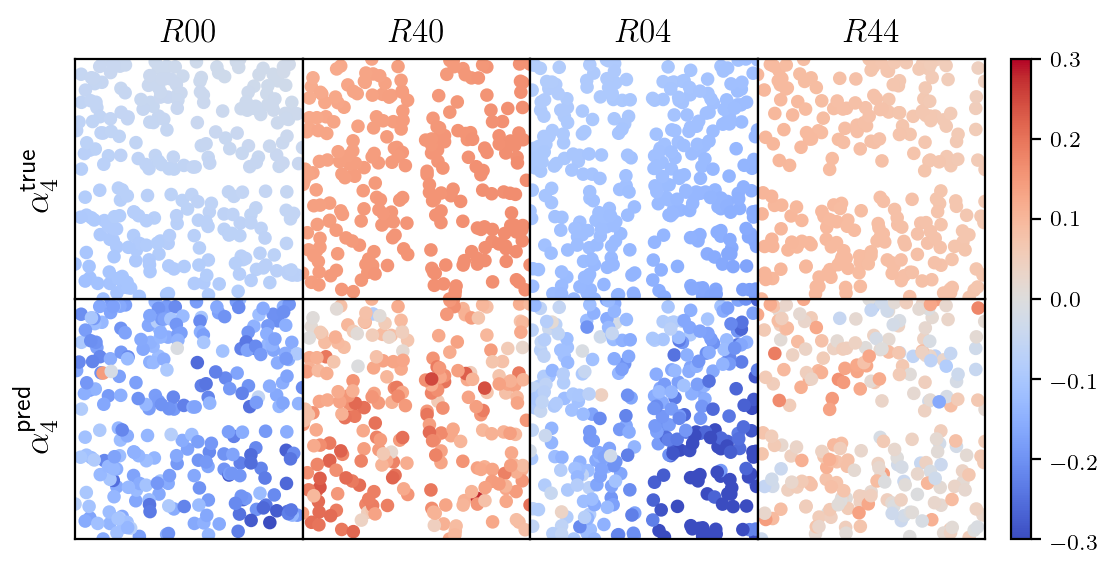
\includegraphics[width=\textwidth]{figs/interp/rafts.png}
\end{tabular}
\end{center}
\caption[Todo]{Todo.\label{fig:rafts}}
\end{figure}

\begin{figure}[!htbp]
\begin{center}
\begin{tabular}{c}
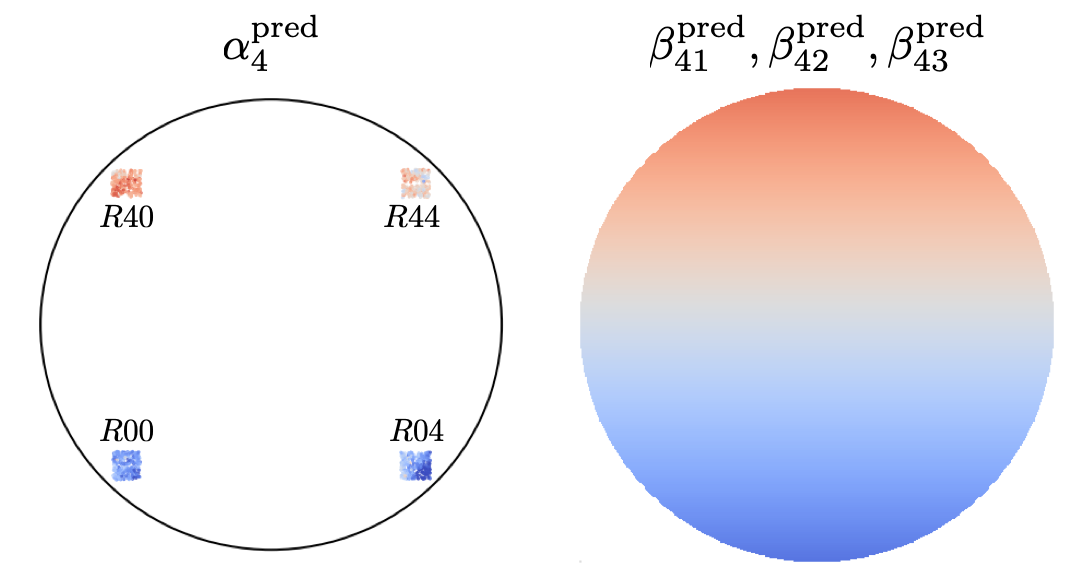
\includegraphics[width=\textwidth]{figs/interp/fieldols.png}
\end{tabular}
\end{center}
\caption[Todo]{Todo.\label{fig:ls-intuition}}
\end{figure}

\section{Evaluating Different Interpolation Strategies}

\begin{table}
{
\begin{center}
\begin{tabular}{|c|c|c|c|r|}
\hline
 & Median &  & \multicolumn{1}{|c|}{\% Samples} & \multicolumn{1}{|c|}{Relative}  \\
Select & Reduce & Fit & \multicolumn{1}{|c|}{Improved} & \multicolumn{1}{|c|}{Residual} \\
\hline
 &  & $\ell_1$ & $ 99.6$ & $ 0.48 \pm  0.13$\\
Stars & & $\ell_2$ &  $ 99.8$ & $ 0.49 \pm  0.12$\\
and&  & $\ell_{\text{h}}$ &  $ 100.0$ & $ 0.48 \pm  0.12$\\
Blends& \checkmark & $\ell_{1}$ &  $ 97.8$ & $ 0.67 \pm  0.14$\\
& \checkmark & $\ell_{2}$ &  $ 100.0$ & $ 0.46 \pm  0.12$\\ 
\hline
&   & $\ell_1$ &  $ 99.8$ & $ 0.44 \pm  0.11$\\ 
&   & $\ell_2$ &  $ 100.0$ & $ 0.43 \pm  0.10$\\ 
Stars&  & $\ell_{\text{h}}$ &  $ 100.0$ & $ 0.43 \pm  0.10$\\
& \checkmark  & $\ell_{1}$ &  $ 97.2$ & $ 0.64 \pm  0.14$\\
& \checkmark  & $\ell_{2}$ &  $ 99.8$ & $ 0.41 \pm  0.11$\\
\hline
& & $\ell_1$ &  $ 99.6$ & $ 0.37 \pm  0.13$\\ 
Brightest& & \textcolor{blue}{$\ell_2$} & \textcolor{blue}{$ 100.0$} & \textcolor{blue}{$ 0.34 \pm  0.12$}\\ 
Stars& & $\ell_{\text{h}}$ &  $100.0$ & $ 0.34 \pm  0.12$\\ 
& \checkmark & $\ell_{1}$ &  $97.2$ & $ 0.60 \pm  0.16$\\ 
& \checkmark & $\ell_{2}$ &  $100.0$ & $ 0.35 \pm  0.12$\\
\hline
& & $\ell_1$ &  $ 100.0$ & $ 0.13 \pm  0.05$\\ 
Labels & & \textcolor{yellow}{$\ell_2$} & \textcolor{yellow}{$ 100.0$} & \textcolor{yellow}{$ 0.06 \pm  0.02$}\\
& & $\ell_{\text{h}}$ &  $ 100.0$ & $ 0.08 \pm  0.04$\\ 
\hline
\end{tabular}
\end{center}
}
\caption{\textbf{Optics wavefront results on different select-reduce-fit variations.} Each row contains the results for a different combination of select, reduce, and fit steps. The penultimate column contains the percentage of the number of samples where the residual improved. The final column contains the relative residual: the total magnitude of the residual divided by the total magnitude of the true wavefront. The best variation on neural network estimates is highlighted in \textcolor{blue}{blue}. The best variation on the true label estimates is highlighted in \textcolor{yellow}{gold}.}
\label{tab:variations}
\end{table}


\begin{figure}[!htbp]
\begin{center}
\begin{tabular}{c}
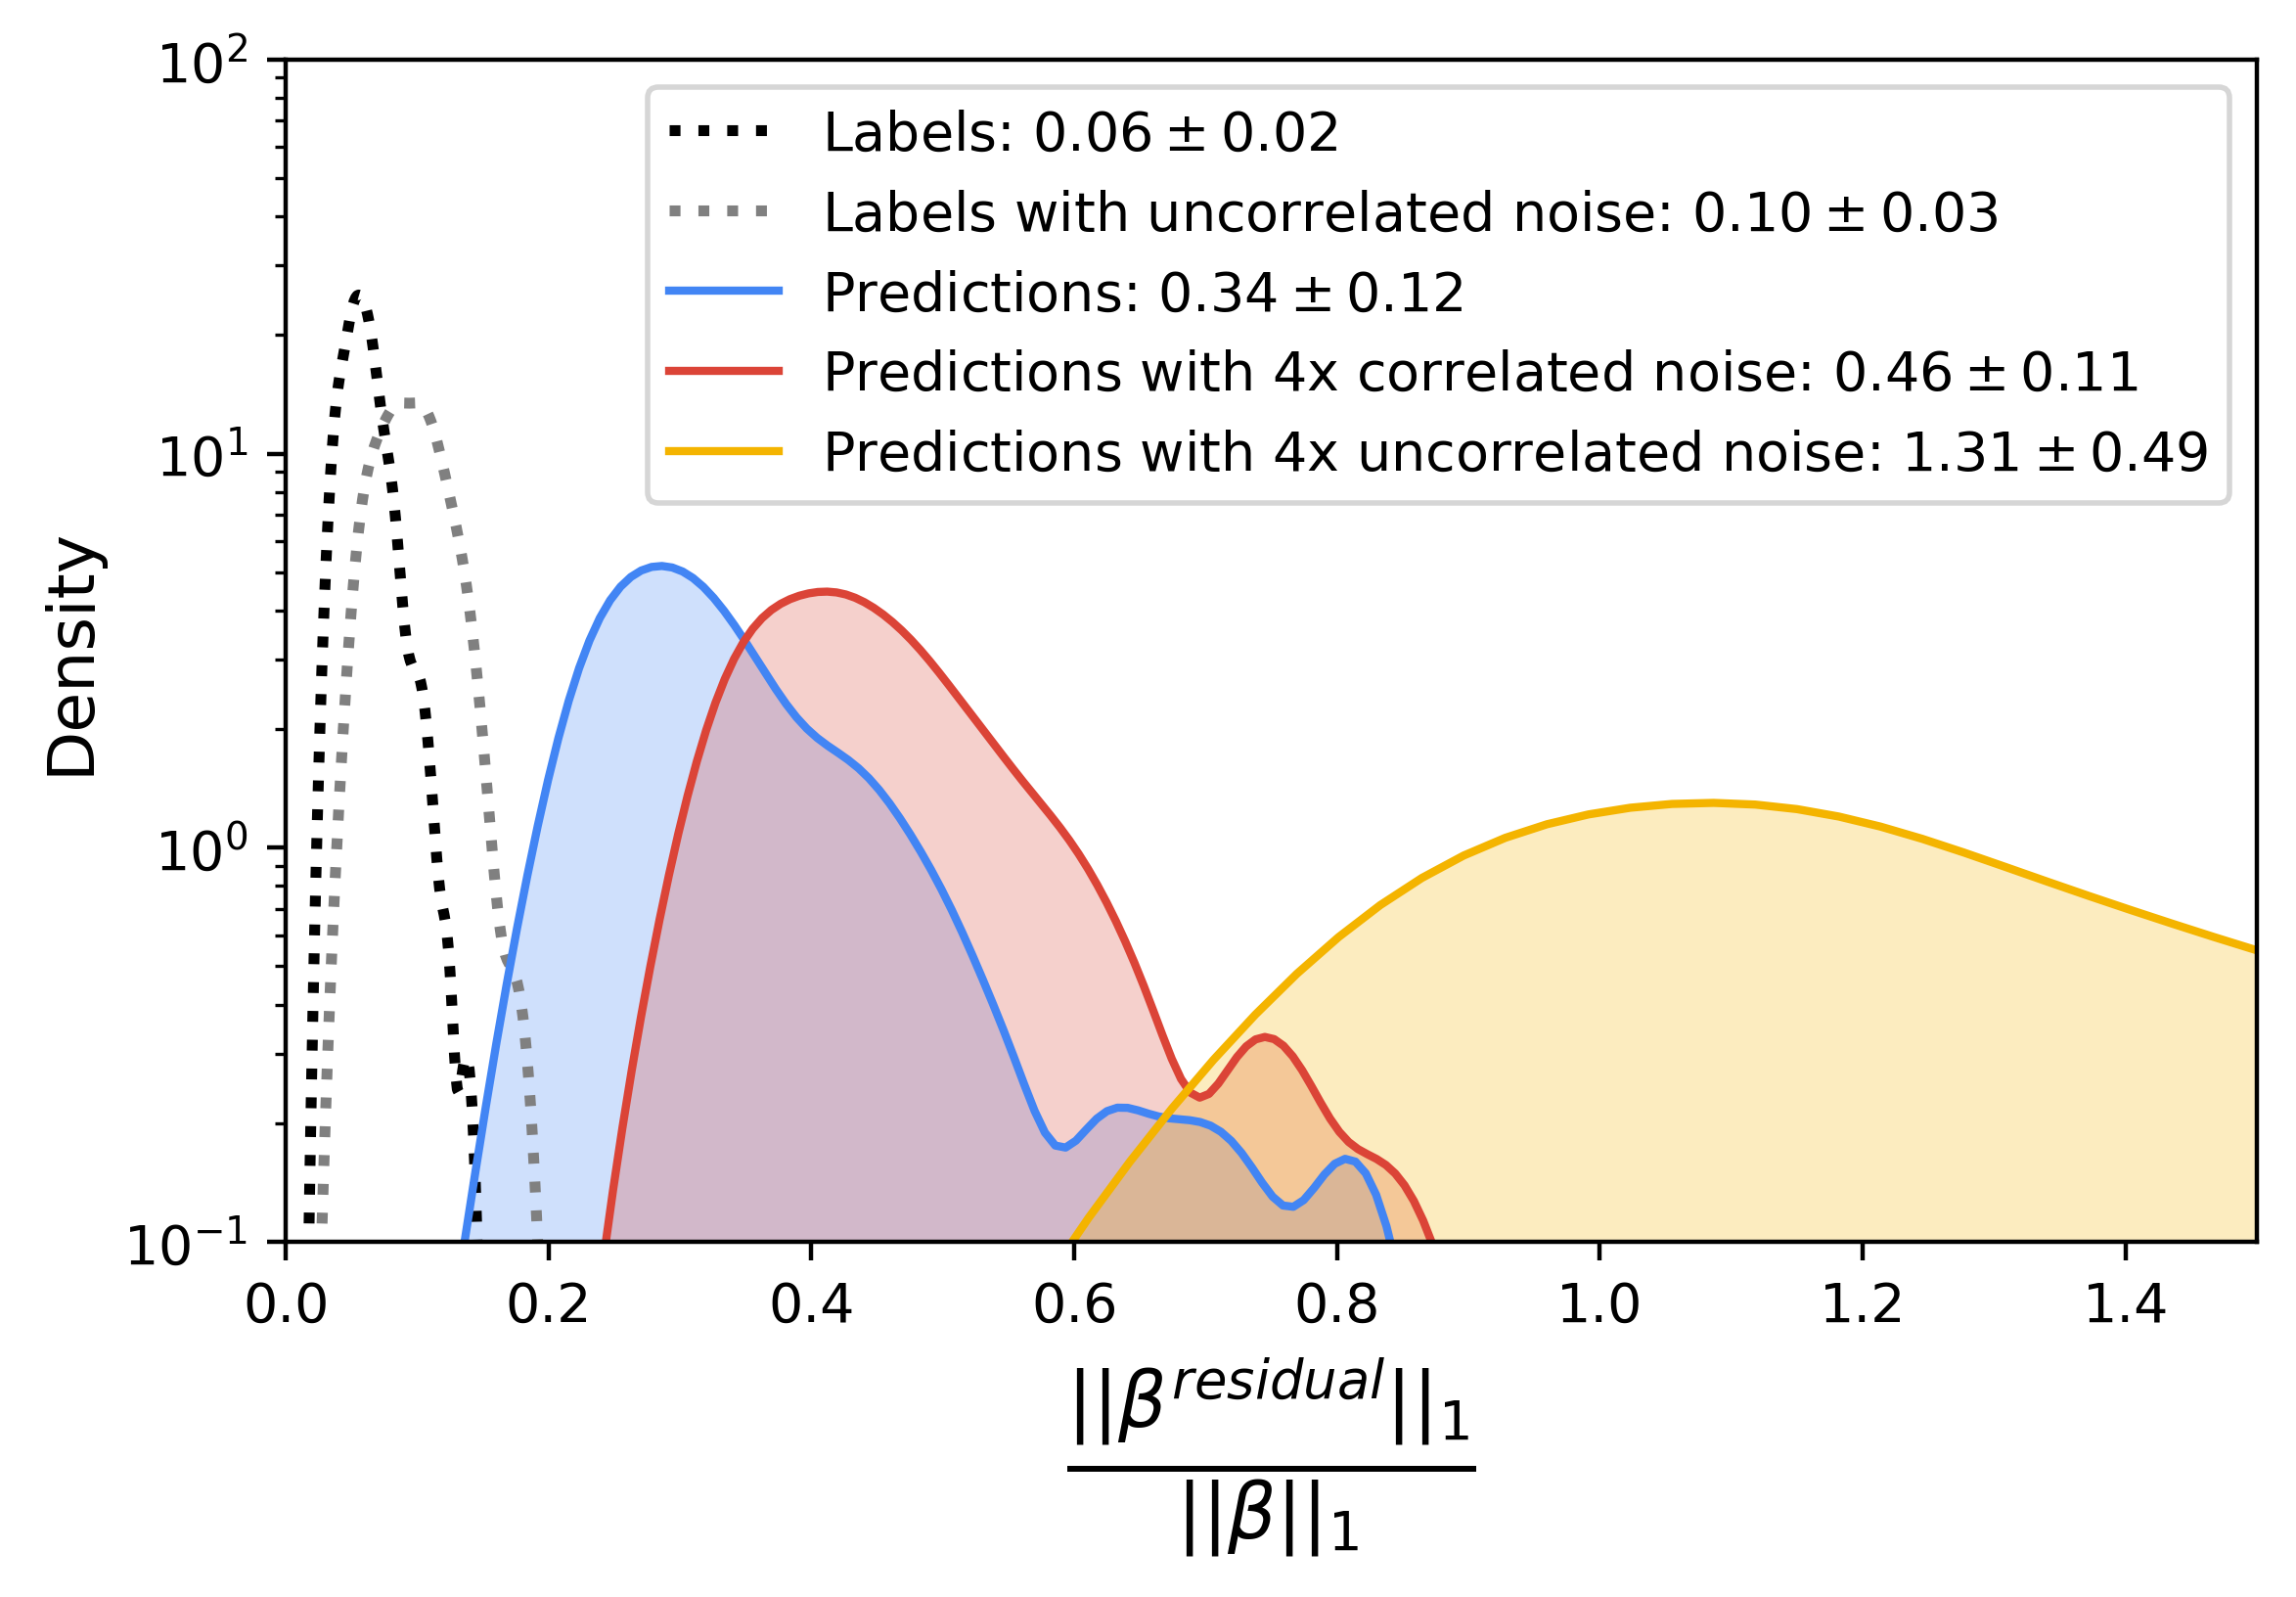
\includegraphics[width=\textwidth]{figs/interp/dist_defense.png}
\end{tabular}
\end{center}
\caption[Todo]{Todo.\label{fig:beta-results}}
\end{figure}


\section{Image Quality Results}

\begin{table}
{
    \begin{center}
    \begin{tabular}{|l|l|c|c|}
    \hline
    State & Position & FWHM & Strehl\\
    \hline
    Before & Center & $0.288 \pm 0.034$ & $0.093 \pm 0.39$ \\
    After & Center & $0.211 \pm 0.005$ &  $0.555 \pm 0.207$\\
    \hline
    Before & Corner & $0.314 \pm 0.045$ & $0.074 \pm 0.32$\\
    After & Corner & $0.215 \pm 0.009$ & $0.400 \pm 0.184$\\
    \hline
    \end{tabular}
    \end{center}
}
\caption{\textbf{Improvement in the optics PSF FWHM and Strehl ratio.} We measure the optics PSF FWHM and Strehl ratio on the original optics wavefront from the observation (Before), and the residual wavefront resulting from subtracting our wavefront estimate from the original optics wavefront (After). The Center position is at the center of the Rubin focal plane; the Corner position is at the center of the $R00$ wavefront sensor in the corner of the focal plane.}
\label{tab:corrections}
\end{table}

\begin{figure}[!htbp]
\begin{center}
\begin{tabular}{c}
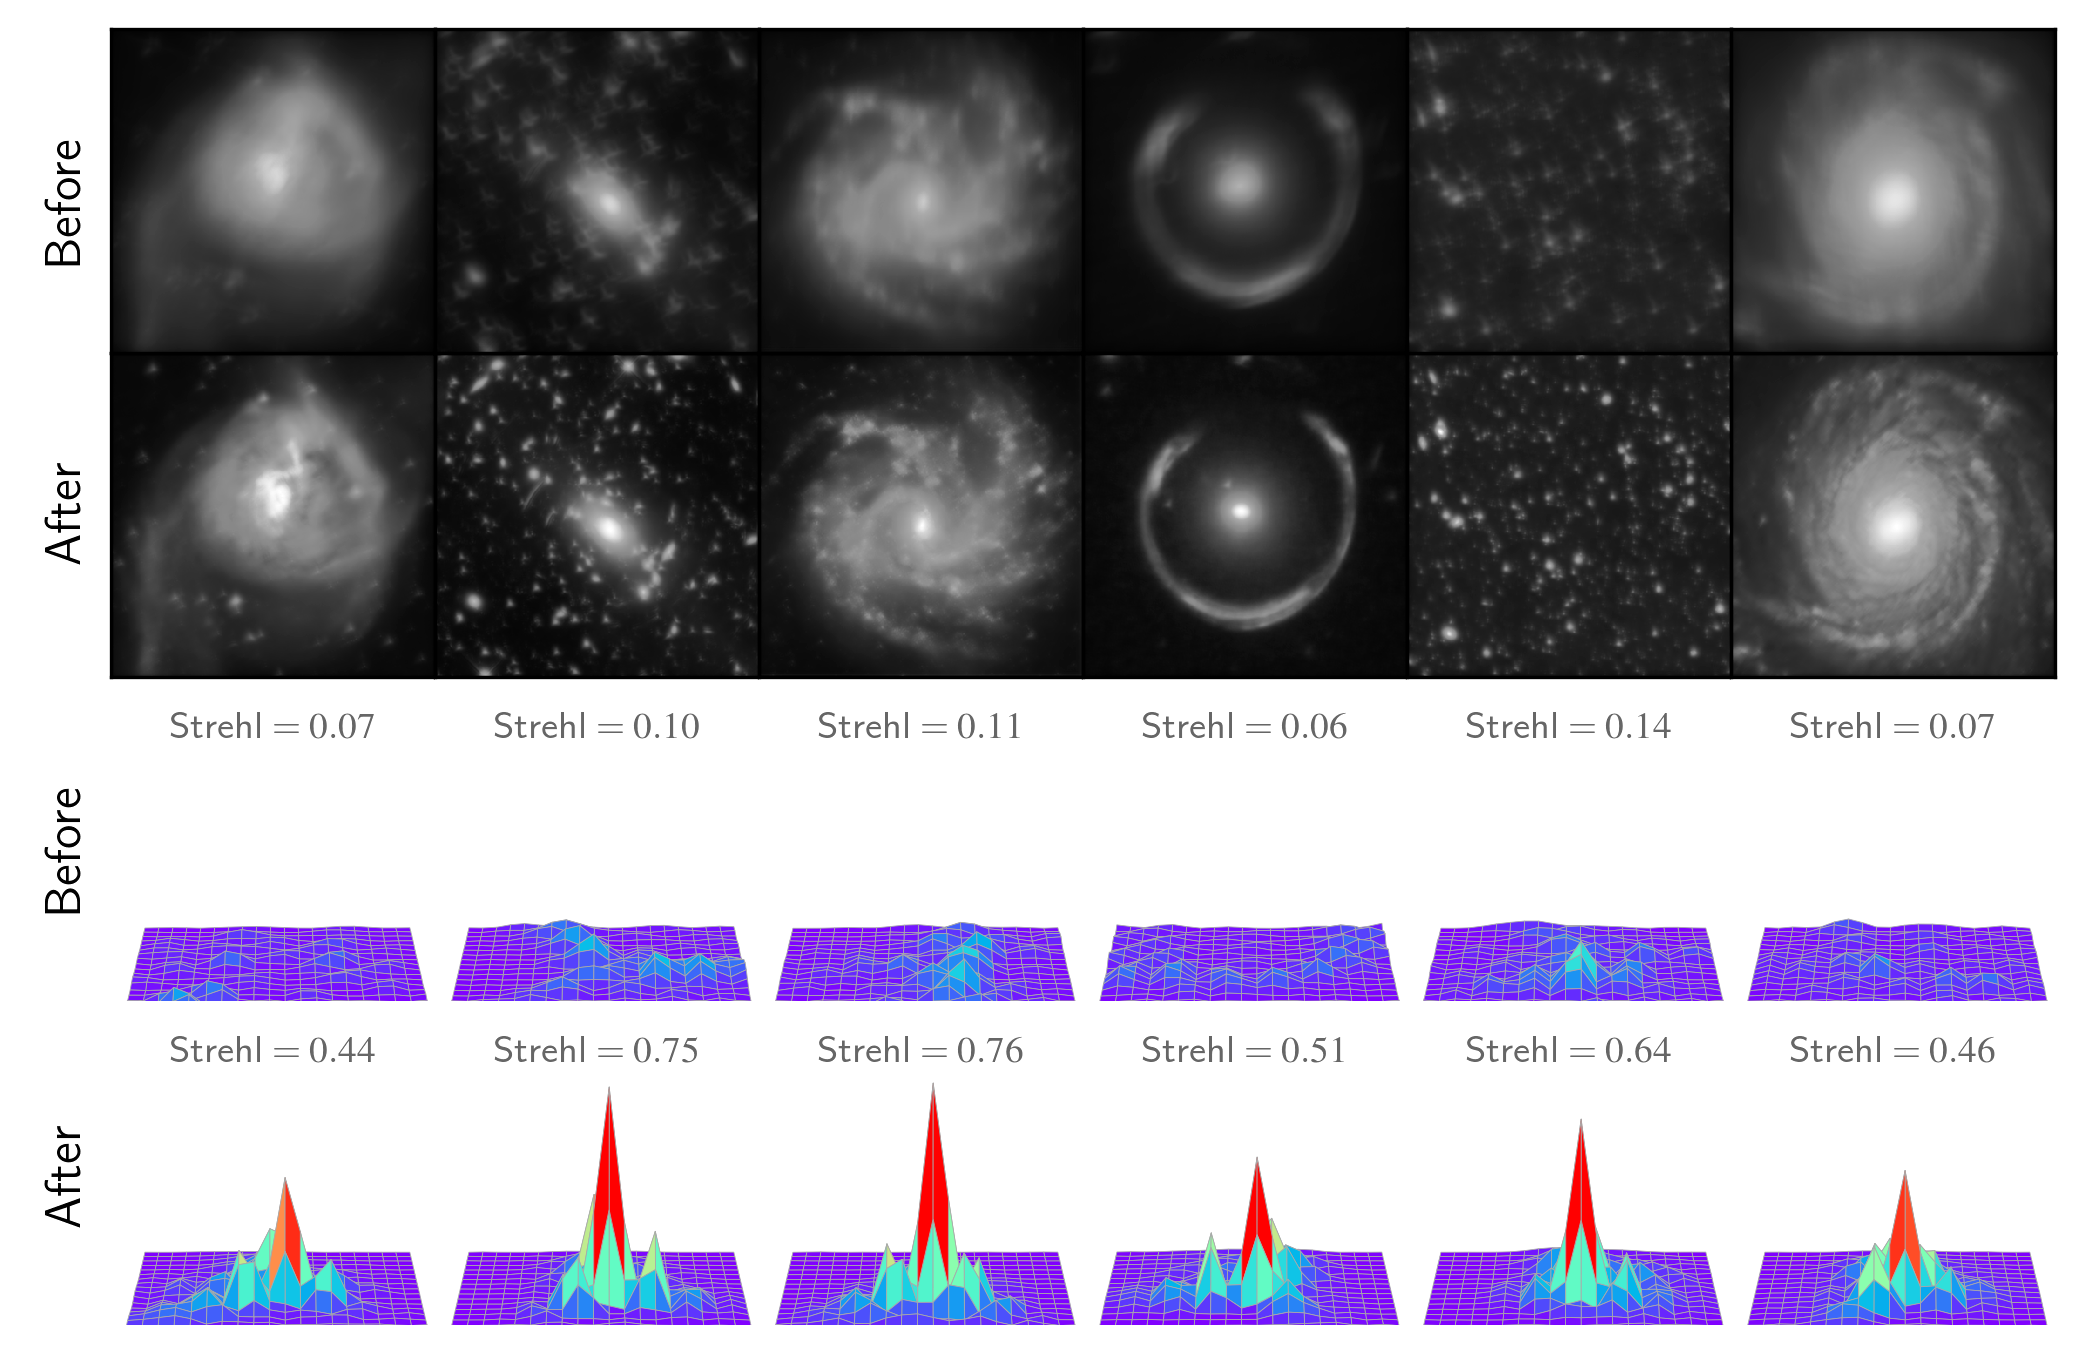
\includegraphics[width=\textwidth]{figs/interp/results.png}
\end{tabular}
\end{center}
\caption[Todo]{\textbf{Hubble Telescope images before and after subtracting the optics wavefront estimated by our framework.} An illustration of the effect of wavefront correction using our techniques on image resolution.  We use actual Hubble Space Telescope images to show the effect.  The Before images are degraded by the wavefront aberrations we have simulated.  The After images show their reconstruction after wavefront estimation and correction using the technique we describe in this paper. On the bottom two rows, we show the effective PSF, both before and after wavefront correction. The images have an angular extent of 3 arcseconds and the PSFs are displayed on a $0.16 \times 0.16$ arcsecond grid. \label{fig:results}}
\end{figure}